%% Dokumentenklasse (Koma Script)
\documentclass[%
   %draft,     % Entwurfsstadium
   final,      % fertiges Dokument
%%%% --- Schriftgröße ---
   11pt,
%%%% --- Sprache ---
   english,
   ngerman,           % Letzte Sprache ist die Hauptsprache, andere muss erst ausgewählt werden.
%%%% === Seitengröße ===
   a4paper,
%%%% === Optionen für den Satzspiegel ===
   %BCOR5mm,         % Zusaetzlicher Rand auf der Innenseite (Bindekorrektur)
   %DIV11,           % Seitengroesse (siehe Koma Skript Dokumentation!)
   %DIVcalc,         % automatische Berechnung einer guten Zeilenlaenge
   1.1headlines,     % Zeilenanzahl der Kopfzeilen
   %headinclude,     % Kopf einbeziehen
   headinclude=false,      % Kopf nicht einbeziehen
   %footinclude,     % Fuss einbeziehen
   footinclude=false,      % Fuss nicht einbeziehen
   %mpinclude,       % Margin einbeziehen
   mpinclude=false,        % Margin nicht einbeziehen
   pagesize,         % Schreibt die Papiergroesse in die Datei.
                     % Wichtig fuer Konvertierungen
%%%% === Layout ===
   oneside,          % einseitiges Layout
   %twoside,         % Seitenraender für zweiseitiges Layout
   onecolumn,        % Einspaltig
   %twocolumn,       % Zweispaltig
   %openany,         % Kapitel beginnen auf jeder Seite
   %openright,        % Kapitel beginnen immer auf der rechten Seite
                     % (macht nur bei 'twoside' Sinn)
   %cleardoubleplain,    % leere, linke Seite mit Seitenstil 'plain'
   %cleardoubleempty,    % leere, linke Seite mit Seitenstil 'empty'
   titlepage,        % Titel als einzelne Seite ('titlepage' Umgebung)
   %notitlepage,     % Titel in Seite integriert
%%%% --- Absatzeinzug ---
   %                 % Absatzabstand: Einzeilig,
   %parskip,         % Freiraum in letzter Zeile: 1em
   %parskip*,        % Freiraum in letzter Zeile: Viertel einer Zeile
   %parskip+,        % Freiraum in letzter Zeile: Drittel einer Zeile
   %parskip-,        % Freiraum in letzter Zeile: keine Vorkehrungen
   %                 % Absatzabstand: Halbzeilig
   %halfparskip,     % Freiraum in letzter Zeile: 1em
   %halfparskip*,    % Freiraum in letzter Zeile: Viertel einer Zeile
   %halfparskip+,    % Freiraum in letzter Zeile: Drittel einer Zeile
   parskip=half,      % Freiraum in letzter Zeile: keine Vorkehrungen
   %                 % Absatzabstand: keiner
   %parindent,       % Eingerückt (Standard)
%%%% --- Kolumnentitel ---
   headsepline,      % Linie unter Kolumnentitel
   %headnosepline,   % keine Linie unter Kolumnentitel
   %footsepline,     % Linie unter Fussnote
   %footnosepline,   % keine Linie unter Fussnote
%%%% --- Kapitel ---
   %chapterprefix,   % Ausgabe von 'Kapitel:'
   chapterprefix=false,
   version=first,  % keine Ausgabe von 'Kapitel:'
%%%% === Verzeichnisse (TOC, LOF, LOT, BIB) ===
   listof=totoc,      % Tabellen & Abbildungsverzeichnis ins TOC
   %idxtotoc,        % Index ins TOC
   bibliography=totoc,
   verson=first,         % Bibliographie ins TOC
   %bibtotocnumbered, % Bibliographie im TOC nummeriert
   %liststotocnumbered, % Alle Verzeichnisse im TOC nummeriert
   toc=graduated,        % eingereuckte Gliederung
   %tocleft,         % Tabellenartige TOC
   %listsindent,      % eingereuckte LOT, LOF
   %listsleft,       % Tabellenartige LOT, LOF
   %pointednumbers,  % Überschriftnummerierung mit Punkt, siehe DUDEN !
   %pointlessnumbers, % Überschriftnummerierung ohne Punkt, siehe DUDEN !
   %openbib,         % alternative Formatierung des Literaturverzeichnisses
%%%% === Matheformeln ===
   %leqno,           % Formelnummern links
   fleqn,            % Formeln werden linksbuendig angezeigt
]{scrbook}%     Klassen: scrartcl, scrreprt, scrbook
% -------------------------------------------------------------------------

% -------------- Daten f�r die Titelseite --> diese m�ssen angepasst werden!
\newcommand*{\thedockind}{Bachelorarbeit}
\newcommand*{\thetitle}{Evaluierung einer Amazon Web Services L�sung zur Erfassung und Verarbeitung von Sensordaten}
\newcommand*{\thesubtitle}{}
\newcommand*{\theauthor}{Hendrik Hagmans}
\newcommand*{\thematriculationnumber}{7082973} % Matrikelnummer
\newcommand*{\thebirthday}{02.04.1992} % Geburtstag
\newcommand*{\themajor}{SWT Dual} % Studiengang
\newcommand*{\thedate}{\today} % \today kann durch ein Datum erstetzt werden.
\newcommand*{\thebetreuer}{Prof. Dr. Martin Hirsch}
\newcommand*{\thezweitbetreuer}{Prof. Dr. Sabine Sachweh}
% -------------- Ende Daten f�r die Titelseite


%%% Doc: ftp://tug.ctan.org/pub/tex-archive/macros/latex/required/babel/babel.pdf
% Languagesetting
\usepackage{babel}	% Sprache

\usepackage{textpos} 

\usepackage{tabularx}

\usepackage{courier}

\usepackage{textcomp}

\usepackage{fixltx2e}	% Verbessert einige Kernkompetenzen von LaTeX2e
\usepackage{ellipsis}	% Korrigiert den Wei�raum um Auslassungspunkte

\usepackage{placeins} 

\usepackage{ifpdf}
\ifpdf
\pdfinfo {
	/Author (\theauthor)
	/Title (\thetitle)
	/Subject ()
	/Keywords ()
%	/CreationDate (D:YYYYMMTTHHMMSS)
}
\fi



%%% Doc: www.cs.brown.edu/system/software/latex/doc/calc.pdf
% Calculation with LaTeX
\usepackage{calc}

%%% Doc: ftp://tug.ctan.org/pub/tex-archive/macros/latex/contrib/xcolor/xcolor.pdf
% Farben
% Incompatible: Do not load when using pstricks !
\usepackage[
	table % Load for using rowcolors command in tables
]{xcolor}

\usepackage{tikz}
\usetikzlibrary{% 
   arrows,% 
   calc,% 
   fit,% 
   patterns,% 
   plotmarks,% 
   shapes.geometric,% 
   shapes.misc,% 
   shapes.symbols,% 
   shapes.arrows,% 
   shapes.callouts,% 
   shapes.multipart,% 
   shapes.gates.logic.US,% 
   shapes.gates.logic.IEC,% 
   er,% 
   automata,% 
   backgrounds,% 
   chains,% 
   topaths,% 
   trees,% 
   petri,% 
   mindmap,% 
   matrix,% 
   calendar,% 
   folding,% 
   fadings,% 
   through,% 
   positioning,% 
   scopes,% 
   decorations.fractals,% 
   decorations.shapes,% 
   decorations.text,% 
   decorations.pathmorphing,% 
   decorations.pathreplacing,% 
   decorations.footprints,% 
   decorations.markings,% 
   shadows} 
   
%%% Doc: ftp://tug.ctan.org/pub/tex-archive/macros/latex/required/graphics/grfguide.pdf
% Bilder
\usepackage[%
	%final,
	%draft % do not include images (faster)
]{graphicx}


% bessere Abstaende innerhalb der Tabelle (Layout))
% -------------------------------------------------
%%% Doc: ftp://tug.ctan.org/pub/tex-archive/macros/latex/contrib/booktabs/booktabs.pdf
\usepackage{booktabs}


%%% Doc: ftp://tug.ctan.org/pub/tex-archive/macros/latex/contrib/enumitem/enumitem.pdf
% Better than 'paralist' and 'enumerate' because it uses a keyvalue interface!
% Do not load together with enumerate.
%\usepackage{enumitem}

\usepackage{paralist}


%%% Doc: http://www.ctan.org/tex-archive/macros/latex/contrib/acronym/acronym.pdf
% Usage:
%        Definition: \acro{ acronym }[ short name ]{ full name }
%        Nutzung im Text: \ac{acronym}
 \usepackage[
 	footnote,	% Full names appear in the footnote
 	%smaller,		% Print acronym in smaller fontsize
 	%printonlyused %
 ]{acronym}
%\chapter*{Abk�rzungsverzeichnis}
\begin{acronym}[BiPRO ] %L�ngster Begriff
\setlength{\itemsep}{-\parsep}
	\acro{AWS}{Amazon Web Services}
	\acro{EC2}{Amazon Elastic Compute Cloud}
	\acro{ECS}{Amazon EC2 Container Service }
	\acro{HTTP}{Hypertext Transfer Protocol}
	\acro{IoT}{Internet of Things}
	\acro{RDS}{Amazon Relational Database Service}
	\acro{REST}{Representational State Transfer}
	%usw.
\end{acronym}



%% Kopf und Fusszeilen====================================================
%%% Doc: ftp://tug.ctan.org/pub/tex-archive/macros/latex/contrib/koma-script/scrguide.pdf
\usepackage[%
   automark,         % automatische Aktualisierung der Kolumnentitel
   %nouppercase,      % Grossbuchstaben verhindern
   %markuppercase    % Grossbuchstaben erzwingen
   %markusedcase     % vordefinierten Stil beibehalten
   %komastyle,       % Stil von Koma Script
   %standardstyle,   % Stil der Standardklassen
]{scrpage2}



%% UeberSchriften (Chapter und Sections) =================================
% -- Ueberschriften komlett Umdefinieren --
%%% Doc: ftp://tug.ctan.org/pub/tex-archive/macros/latex/contrib/titlesec/titlesec.pdf
\usepackage{titlesec}

% -- Section Aussehen veraendern --
% --------------------------------
%% -> Section mit Unterstrich
% \titleformat{\section}
%   [hang]%[frame]display
%   {\usekomafont{sectioning}\Large}
%  {\thesection}
%   {6pt}
%   {}
%   [\titlerule \vspace{0.5\baselineskip}]
% --------------------------------

% -- Chapter Aussehen veraendern --
% --------------------------------
\titleformat{\chapter}[block]	% {command}[shape]
  {\usekomafont{chapter}\huge\sffamily\bfseries}	% format
  {   										% label
  {\thechapter.} \filright%
  }%}
  {1pt}										% sep (from chapternumber)
  {\vspace{0.5pc} \filright}   % {before}[after] (before chaptertitle and after)
  [\vspace{0.5pc} \filright {}]

% \titleformat{\chapter}[]%
%    {\usekomafont{chapter}\huge\sffamily\bfseries}%
%    {\thechapter}%
%    {1em}%
%    {}%


\usepackage{rotating}


\usepackage[numbers,square]{natbib}
%\usepackage{cite}
%\bibliographystyle{dinat}
%\citestyle{alpha}
\bibliographystyle{alpha}


% Quotes =================================================================
%% Doc: ftp://tug.ctan.org/pub/tex-archive/macros/latex/contrib/csquotes/csquotes.pdf
% Advanced features for clever quotations
\usepackage[%
   babel,            % the style of all quotation marks will be adapted
                     % to the document language as chosen by 'babel'
   german=quotes,		% Styles of quotes in each language
   %german=guillemets,
   english=british,
   french=guillemets
]{csquotes}
%\usepackage{floatflt}

\usepackage{wrapfig}

%\usepackage{subfigure}

\usepackage{blindtext}

\usepackage{listings}
\definecolor{lila}{RGB}{112, 6, 147}
\definecolor{kommentgreen}{RGB}{5,132,71}
\definecolor{grey}{RGB}{242,242,242}  
\definecolor{darkgreen}{named}{green}
\definecolor{darkblue}{named}{blue}
\definecolor{lightblue}{RGB} {63,95,191}
\definecolor{darkred}{named}{red}
\definecolor{grau}{named}{gray}
\definecolor{fh_orange}{rgb}{0.953,0.201,0}
\definecolor{fh_grau}{rgb}{0.76,0.75,0.76}

\definecolor{listinggray}{gray}{0.9}
\definecolor{lbcolor}{rgb}{0.9,0.9,0.9}

\lstset{
	tabsize=3,
	float=tbph,
	frame=single,
	extendedchars,
	breaklines=true,
	basicstyle=\fontsize{9pt}{9pt}\selectfont,
	columns=flexible, %ist notwendig, damit man Quelltext aus den Listings kopieren kann
	numbers=left, 
	numberstyle=\color{black},
	captionpos=b,
	aboveskip=7mm,
	backgroundcolor=\color{grey}
}

\lstdefinestyle{java}
{
	language=Java,
	keywordstyle=\color{lila},  	% underlined bold black keywords 
	identifierstyle=\color{blue}, 
	commentstyle=\color{kommentgreen}, % white comments 
	stringstyle=\color{black},
}

\lstdefinestyle{xml}
{
	language=xml,
	basicstyle=\fontsize{9pt}{9pt}\selectfont\color{kommentgreen},
	keywordstyle=\color{lila},  	% underlined bold black keywords 
	%Hier k�nnen bei Bedarf noch weitere Keywords eingetragen werden
	keywords={name, value, version, encoding, id, type, xmlns:xsi, ref, namespace},
	identifierstyle=\color{black},  
	stringstyle=\color{blue},  
	commentstyle=\color{lightblue},
	morecomment=[s]{<!--}{-->},
	rulecolor=\color{black}
}

\usepackage{multicol}

\usepackage{nameref}

\usepackage{hyperref}
\hypersetup{breaklinks=true}
\hypersetup{colorlinks=true,linkcolor=black,urlcolor=black,citecolor=black}
%\hypersetup{frenchlinks}	% Use small caps instead of color for links
%\hypersetup{pdfpagemode=FullScreen}
%\hypersetup{pdfstartpage=3}
%\hypersetup{pdfstartview=Fit}


% Tabellen ueber mehere Seiten
% ----------------------------
%%% Doc: ftp://tug.ctan.org/pub/tex-archive/macros/latex/contrib/carlisle/ltxtable.pdf
% \usepackage{ltxtable} % Longtable + tabularx
                        % (multi-page tables) + (auto-sized columns in a fixed width table)
% -> nach hyperref laden
%\usepackage{ltxtable}
%\usepackage{longtable}
\usepackage{tabulary}


% Schusterjunge und Hurenkinder verhindern
\clubpenalty=1000
\widowpenalty=1000
\displaywidowpenalty=1000

% Trennen von Bindestrich oder so ...
%\defaulthyphenchar=127

\usepackage[latin1]{inputenc}
\usepackage[T1]{fontenc}
\usepackage{alltt}
\usepackage{marvosym}
\usepackage{fancybox}
\usepackage[hang,small,bf]{caption}
\usepackage{float} 
\usepackage{multirow}

\lstset{basicstyle=\footnotesize\ttfamily,breaklines=true}
\lstset{framextopmargin=50pt,frame=bottomline}
\addtokomafont{caption}{\sffamily\small}
\setkomafont{captionlabel}{\sffamily\small}

\newcommand{\keyword}[1]{\textbf{#1}}
%\newcommand{\filename}[1]{\texttt{#1}}
\newcommand{\inlinecode}[1]{\lstinline!#1!}


% Umbenennung von "Listings"
\addto\captionsngerman{%
  \renewcommand{\lstlistlistingname}{Quelltextverzeichnis}%
  \renewcommand{\lstlistingname}{Quelltext}%
  \renewcommand{\}}{}
}

\usepackage{blindtext}
\usepackage{helvet}	%Paket f�r die Schriftart

\renewcommand{\familydefault}{\sfdefault}	%sorgt f�r einheitliche Schriftart im gesamten Dokument
\setcounter{secnumdepth}{5} %legt die Ebene fest, bis zu der nummeriert wird
\setcounter{tocdepth}{5} %legt fest wieviele Ebenen im Inhaltsverzeichnis vorkommen


\begin{document}

	%\captionsetup[figure]{singlelinecheck=false} %sorgt f�r eine Linksb�ndige Bildunterschrift
	%\captionsetup[lstlisting]{singlelinecheck=off}
	\captionsetup{singlelinecheck=off}
	
  	\sffamily		% Schriftart Serifenlos w�hlen
  	\linespread {1.25}\selectfont %Zeilenabstand: 1.25 da er von Haus aus 1.2 ist und 1,25 * 1,2 = 1,5

	%Titelseite einf�gen
	
\begin{titlepage}
		
%%%%%%%%%%%%%%%%%%%%%%%%%%%%%% -*- Mode: Latex -*- %%%%%%%%%%%%%%%%%%%%%%%%%%%%
%% 
%% pa_ba_titelblatt.tex 
%% 
%% Copyright (C) 2008 Alexander Sprack / Claudia Holz
%% 
%%%%%%%%%%%%%%%%%%%%%%%%%%%%%%%%%%%%%%%%%%%%%%%%%%%%%%%%%%%%%%%%%%%%%%%%%%%%%%%
  \begin{textblock}{6.5}(-1,-3)
    \begin{color}{fh_grau}
      \rule{6.8cm}{33cm}    
    \end{color}
  \end{textblock}
  \begin{textblock}{6.5}(-1.2,-0.7)
%  \includegraphics[width=3.8cm]{my-fh-logo}% selbst basteln, falls gew�nscht! 
                                            % Das offizielle Logo ist nicht
                                            % gestattet!! Bitte BEACHTEN!!!
  \end{textblock}
  \begin{textblock}{6.5}(-0.8,1)
    {\Large \textsf{\thedockind}}            
  \end{textblock}

  \begin{textblock}{7}(4.5,2)
    {\noindent \huge 
      \textsf{\textbf{Evaluierung einer Amazon Web Services\textcopyright{} L�sung zur Erfassung und Verarbeitung von Sensordaten\\[0.3cm] 
          \Large  \thesubtitle\\[0.05cm]
          }} }
  \end{textblock}


  \begin{textblock}{6}(4.5,6.5)\noindent
    \textsf{An der Fachhochschule Dortmund\\
    im Fachbereich Informatik\\
    Studiengang \themajor \\
    erstellte Thesis zur Erlangung des akademischen Grades Bachelor of Science B. Sc.  \\
   }
  \end{textblock}

  \begin{textblock}{6.5}(-0.4,10.0)
    \noindent
    \textsf{von \\
      \theauthor \\
      geb.\ am \thebirthday  \\
      Matr.-Nr. \thematriculationnumber\\[0.7cm]
      Betreuer:\\
       \noindent\hspace*{6mm} \thebetreuer \\
       \noindent\hspace*{6mm} \thezweitbetreuer\\ [0.5cm]
      Dortmund, \today}    
  \end{textblock}
	

\end{titlepage}



%\thispagestyle{empty}

	
	\thispagestyle{empty} % Seitennummerierung fuer diese Seite unterbinden

\section*{Zusammenfassung}
\label{sec:Zusammenfassung}
Amazon Web Services gibt es nun schon seit einigen Jahren und bietet verschiedenste Cloud Services f�r unterschiedlichste Anforderungen. Amazon Web Services unter- scheidet sich von vielen anderen Anbietern vor allem durch die variable Leistungsabrechnung und die Vielfalt der Angebote. In dieser Arbeit soll nun mittels eines Beispiels evaluiert werden, ob Amazon Web Services auch f�r gro�e Datenstr�me wie beispielsweise Sensordaten geeignet ist.

\section*{Abstract}
\label{sec:Abstract}
Amazon Web Services are present for quite a few years and offer several services for different requirements. The most important differences between Amazon Web Services and other cloud computing providers is flexible service billing and the diversity of their offers. In this work it will be evaluated by means of an example if Amazon Web Services are suitable for use with big data streams like sensor data.

	\frontmatter	 		%r�mische Nummerierung f�r Inhaltsverzeichnis aktivieren
	\tableofcontents	%Inhaltsverzeichnis erstellen
	\mainmatter	 			%Arabische Seitenummerierung

	\pagestyle{scrheadings}
	
	
	% ----------------- Einf�gen des eigentlichen Textes
	
	\chapter{Einleitung}
		\section{Motivation}

Cloud Computing ist ein immer gr��er werdendes Thema in der IT. Immer mehr Daten werden nicht mehr lokal, sondern in der Cloud gespeichert und werden somit f�r jeden �berall verf�gbar. Auch Anwendungen werden immer h�ufiger nicht mehr lokal betrieben, sondern nutzen die gro�en Rechnerleistungen von Cloud L�sungen, um m�glichst skalierbar zu sein und mittels Redundanz h�here Verf�gbarkeiten und bessere Latenzzeiten zu erreichen. Zudem bieten Cloud L�sungen die M�glichkeit, Investitionskosten in Betriebskosten umzuwandeln, da keine neuen Server und andere Ger�te gekauft werden m�ssen, sondern f�r die Nutzung bezahlt wird. Webapplikationen bilden hier keine Ausnahme. Anstatt eigene Rechenzentren aufbauen zu m�ssen, werden Webapplikationen immer h�ufiger bei externen Cloudanbietern betrieben um Kosten und den Administrationsaufwand solcher Systeme zu reduzieren. Ein gro�er Anbieter solcher Plattformen ist Amazon, die mit ihren Amazon Web Services \cite{aws} eine Reihe von Cloud Services bieten, die von vielen weltweit operierenden Unternehmen genutzt wird. Doch wie kann man mittels Amazon Web Services gro�e Datenfl�sse wie beispielsweise die Aufzeichnung von Sensordaten in einem automatisierten Heimsystem am besten verwalten?

\section{Zielsetzung}
Es soll eine Wettersimulation erstellt werden, die aus mehreren Services besteht, die dauerhaft Daten liefern. Beispielsweise mehrere virtuelle Temperatursensoren, die Zufallszahlen innerhalb eines bestimmten Werteintervalls liefern. Die Temperaturwerte k�nnen sich auch gegenseitig beeinflussen. So beeinflusst eine h�here Au�entemperatur auch die Innentemperatur. Diese Komponenten werden jeweils in einem Docker Container \cite{docker} auf Amazon ECS \cite{ecs} deployed und liefern einen konstanten Datenstrom von Temperaturdaten. Der Datenstrom soll skaliert werden k�nnen und bspw. die Daten eines ganzen Tages in einer Stunde erzeugen. Die Daten werden in einer SQL Datenbank auf Amazon RDS \cite{rds} oder Amazon DynamoDB \cite{dynamodb} gespeichert. Eine eigene L�sung mit Apache Cassandra \cite{cassandra} w�re auch m�glich. Im Dashboard soll eine �bersicht der Daten in Verlaufsdiagrammen verf�gbar sein. Hier ist auch eine Anpassung der Zeitskalierung m�glich.
Der Fokus liegt hierbei nicht auf einer akkuraten Wettersimulation, sondern auf der Evaluation der AWS Services f�r gro�e Datenstr�me und der Vergleich zwischen den einzelnen AWS Services. Bspw. k�nnten Teile der Architektur auch mit Amazon Kinesis \cite{kinesis} umgesetzt werden, das speziell f�r gro�e Datenstr�me konzipiert wurde. Hier k�nnte man beide Architekturentw�rfe vergleichen.
Dieses Projekt wurde in einer Projektarbeit bereits geplant und analysiert und soll in dieser Bachelorarbeit nun implementiert werden. Daraufhin soll eine Evaluation der verwendeten AWS Komponenten durchgef�hrt werden.

\section{Vorgehensweise}
\begin{itemize}
	\item Wie wird vorgegangen, um das Ziel zu erreichen?
	\item Warum ist die Arbeit so gegliedert, wie sie gegliedert ist?
	\item Welche Aspekte werden nicht behandelt \textbf{und} warum?
\end{itemize}
	\chapter{Projektplanung}
		Das Projekt wurde bereits in einer vorher bearbeiteten Projektarbeit \cite{projektarbeit} geplant. Dabei wurden mehrere Analysen durchgef�hrt, die in diesem Kapitel vorgestellt werden. Als Ergebnis der Anforderungsanalyse wurde folgende Liste von Anforderungen erstellt:

\begin{table}[h!]
	
	\begin{tabularx}{\textwidth}{|p{\textwidth/100*20}|p{\textwidth/100*50}|X|}
		
		\hline
		
		Thema & Beschreibung & Kano Bewertung \\
		
		\hline
		
		\hline
		
		Dauerhafter Datenstrom & Producer sollen dauerhaft Temperaturdaten liefern & Basismerkmal \\
		
		\hline
		
		Daten Persistenz & Die Daten sollen dauerhaft in einer Datenbank persistiert werden & Basismerkmal \\
		
		\hline
		
		Start und Stopp des Datenstroms & Der Datenstrom soll vom Nutzer gestartet und gestoppt werden k�nnen & Basismerkmal \\
		
		\hline
		
		Datenstrom Skalierung & Der Datenstrom soll skaliert werden k�nnen. Beispielsweise sollen die Daten eines Tages in einer Stunde ausgegeben werden k�nnen & Basismerkmal \\
		
		\hline
		
		Dashboard & Nutzer soll die aktuellen Daten in einem Dashboard einsehen k�nnen & Basismerkmal \\
		
		\hline
		
		Mehrere AWS Services & Die Applikation soll auf mehreren AWS Services deployed werden, um diese vergleichen zu k�nnen & Basismerkmal \\
		
		
		\hline
				Dashboard Darstellung & Die Daten werden im Dashboard in verschiedenen Diagrammen wie bspw. Verlaufsdiagrammen dargestellt sowie in Tabellen. & Leistungsmerkmal \\
				
				\hline
		
	\end{tabularx}
	
	\caption{Anforderungen an das Projekt Teil 1}
	\label{anforderungen_1}
\end{table}

\begin{table}[h!]
	
	\begin{tabularx}{\textwidth}{|p{\textwidth/100*20}|p{\textwidth/100*50}|X|}
		
		\hline
		
		Thema & Beschreibung & Kano Bewertung \\
		
		\hline
		
		\hline
				
		Verf�gbarkeit & Die Services sollen hochverf�gbar sein & Leistungsmerkmal \\
		
		\hline
		
		Aktualit�t der Daten & Die Daten sollen im Dashboard aktuell gehalten werden, auch wenn die Seite nicht neu geladen wird & Begeisterungs-merkmal \\
		
		\hline
		
		Temperaturen beeinflussen sich gegenseitig & Die Temperaturen sollen sich gegenseitig beeinflussen, z.B. bedingt eine h�here Au�entemperatur eine h�here Innentemperatur & Leistungsmerkmal \\
		
		\hline
		
	\end{tabularx}
	
	\caption{Anforderungen an das Projekt Teil 2}
	\label{anforderungen_2}
\end{table}

Die Anforderungsliste ist nach der Priorisierung sortiert, die im Rahmen einer Kano Bewertung der einzelnen Punkte erstellt wurde. Wie in den Tabellen \ref{anforderungen_1} und \ref{anforderungen_2} zu sehen, wurden die Basismerkmale am h�chsten priorisiert, da diese den Erfolg des Projektes ausmachen. Auf der Basis dieser Anforderungsanalyse wurde zudem folgendes Pflichtenheft erstellt:

\begin{table}[h!]

\begin{tabularx}{\textwidth}{|p{\textwidth/100*30}|p{\textwidth/100*50}|X|}

\hline

Thema & Beschreibung & Aufwand \\

\hline

\hline

AWS kennenlernen & Kennenlernen der AWS Services und erste Deployments von Containern & 10 \\

\hline

Docker Image & Docker Image mit allen ben�tigten Ressourcen erstellen & 3 \\

\hline

Docker Container & Docker Container aus dem Image mit der fertigen Applikation erzeugen & 3 \\

\hline

Producer & Es m�ssen mehrere Producer geschrieben werden, die konstant Temperaturdaten liefern. Die Producer werden in Java geschrieben & 20 \\

\hline

Consumer & Es muss mindestens ein Consumer geschrieben werden, der die Daten der Producer verarbeitet. Der Consumer wird in Java geschrieben & 20 \\

\hline

\end{tabularx}

\caption{Pflichtenheft Teil 1}

\end{table}

\begin{table}[h!]

\begin{tabularx}{\textwidth}{|p{\textwidth/100*30}|p{\textwidth/100*50}|X|}
	
	\hline
	
	Thema & Beschreibung & Aufwand \\
	
	\hline
	
	\hline
	
	Consumer DB & Es muss eine Datenbank entweder auf Amazon RDS oder Amazon DynamoDB (oder andere L�sungen bspw. mit Cassandra) eingerichtet werden & 10 \\
	
	\hline
	
	Consumer DB Zugriff & Der Consumer muss die Temperaturdaten in die DB schreiben k�nnen & 10 \\
	
	\hline
	
	Mehrere AWS Services & Die Applikation f�r mehrere AWS Services kompatibel machen und auf mehreren Services deployen & 20 \\
	
	\hline
	
	Dashboard & Es muss ein Dashboard geschrieben werden, das die Temperaturdaten anzeigen kann & 15 \\
	
	\hline
	
	Dashboard Start Stopp & Es muss im Dashboard die Funktion geben den Datenstrom anhalten oder wieder starten zu k�nnen & 3 \\
	
	\hline
		
	Dashboard Zeitskalierung & Es muss im Dashboard die Funktion geben den Datenstrom verschnellern oder verlangsamen zu k�nnen & 7 \\
	
	\hline
	
	Dashboard Diagramme & Die Daten sollten im Dashboard in Form von Diagrammen dargestellt werden & 10 \\
	
	\hline
	
	Dashboard Diagramme Aktualit�t & Die Daten sollten im Dashboard immer aktuell gehalten werden, auch wenn der Nutzer die Seite nicht aktualisiert & 5 \\
	
	\hline
	
	Producer Temperatur Beeinflussung & Die Temperaturwerte der Producer m�ssen sich gegenseitig beeinflussen. Die Producer m�ssen also untereinander kommunizieren und zumindest Wechsel in der Temperaturtendenz interessierten anderen Producern mitteilen. & 10 \\
	
	\hline
	
\end{tabularx}

\caption{Pflichtenheft Teil 2}

\end{table}

Das Pflichtenheft ist genau wie die Anforderungsliste nach der Priorisierung sortiert, die im Rahmen einer Kano Bewertung der einzelnen Punkte erstellt wurde. Genauere Erl�uterungen der einzelnen Anforderungen und Punkte des Pflichtenhefts finden sich in der Projektarbeit. \newline
Des weiteren wurde im Rahmen der Projektplanung eine Risikoanalyse durchgef�hrt, um die gr��ten Risiken des Projekts zu erkennen und dementsprechende Gegenma�nahmen anwenden zu k�nnen. Hierbei haben sich folgende 4 Risiken herausgestellt:

\begin{table}[h!]
	
	\begin{tabularx}{\textwidth}{|p{\textwidth/100*10}|p{\textwidth/100*40}|p{\textwidth/100*15}|p{\textwidth/100*12}|X|}
		
		\hline
		
		Nummer & Risiko & Eintrittswahr-scheinlichkeit in \% & gesch�tzer Schaden in \texteuro & Risiko-faktor  \\
		
		\hline
		
		\hline
		
		1 & AWS Zugriff zu sp�t bekommen & 30 & 300 & 90 \\
		
		\hline
		
		2 & Producer erzeugt zu viele Daten und damit zu viele Kosten bei AWS & 150 & 20 & 75 \\
		
		\hline
		
		3 & Teile des Projekts werden nicht rechtzeitig vor Abgabe erstellt & 10 & 1000 & 100 \\
		
		\hline
		
		4 & Untersch�tzen des Umfangs oder der Schwierigkeit des Projektes & 10 & 1000 & 100 \\
		
		\hline
		
	\end{tabularx}
	
	\caption{Risikoliste}
	
\end{table}

Der Risikofaktor entspricht der Formel \(\frac{Eintrittswahrscheinlichkeit \cdot Schaden}{100}\).Dementsprechend befinden sich gerade die Risiken Nummer 3 und 4 durchaus in einem gef�hrlichen Bereich, der das Projekt gef�hrden k�nnte. In der Projektarbeit wurden allerdings Ma�nahmen zur Verhinderung des Eintretens der Risiken sowie der Verminderung der Kosten bei Eintreten der Risiken ermittelt, die in der Ausf�hrung des Projektes auch umgesetzt wurden.  \newline
Zu guter Letzt wurde eine Kostenplanung erstellt, da die Nutzung von Amazon Web Services Kosten verursachen kann und diese nicht zu hoch ausfallen sollten. Es wurde ein Budget von bis zu 200  \texteuro{} gew�hrt, das nicht �berschritten werden sollte. Daher mussten die aktuellen Kosten st�ndig �berwacht werden. \newline
Im Rahmen der Projektarbeit wurden zudem die Themen und Komponenten, die Teil der Bachelorarbeit sein sollten, behandelt und beschrieben. Darunter z�hlten die Themen Cloud Computing, Amazon Web Services und deren einzelne Komponenten sowie Docker. Daher m�ssen diese Themen in dieser Bachelorarbeit nicht mehr ausf�hrlich behandelt werden. \newline
Eine erste Evaluation der in Frage kommenden Amazon Web Services wurde ebenfalls durchgef�hrt und dabei eine Kombination aus Amazon EC2 als Infrastruktur f�r die Producer und Consumer, Amazon Kinesis als �bertragungskanal f�r die Temperaturdaten sowie Amazon RDS oder Amazon DynamoDB f�r die Persistierung der Daten als passende Services ausgemacht.

	\chapter{Implementierung}
		\section{Projektarchitektur}
Um die Abh�ngigkeitsverwaltung und das Bauen des Projektes m�glichst simpel zu gestalten, wurde f�r das Projekt Apache Maven \cite{maven} genutzt und das Projekt dementsprechend als Maven Projekt erstellt. \newline
Abh�ngigkeiten des Projekts sind der Amazon Kinesis Client in der Version 1.6.1, der Amazon Kinesis Producer in der Version 0.10.2 sowie Eclipse Jetty Servlet \cite{jetty} in der Version 9.2.14.v20151106. \newline
Die Projektarchitektur ist im Grunde genommen genau so, wie sie von Amazon in der Dokumentation von AWS Kinesis vorgestellt wird.

\begin{figure}[!h]

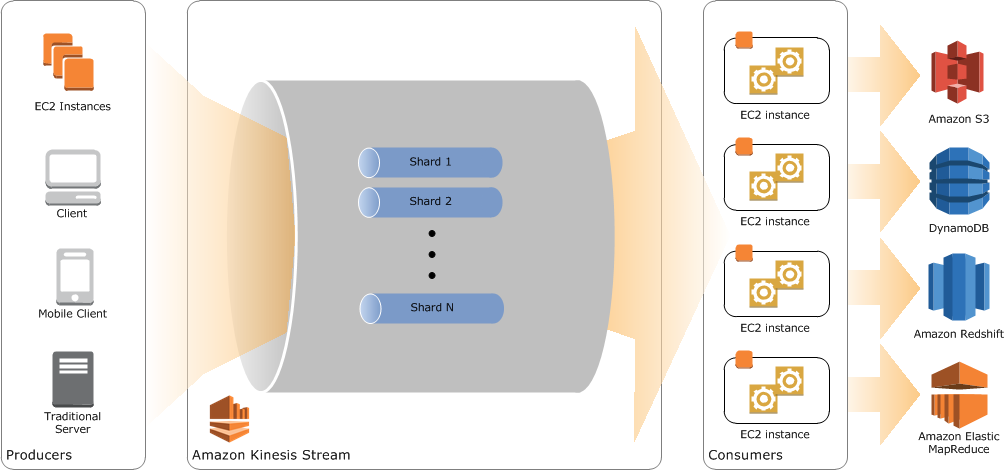
\includegraphics[width=1.0\textwidth]{content/images/kinesis_architecture.png}

\caption{Kinesis Architektur, wie sie von Amazon vorgegeben wird. Quelle: \cite{kinesis_concepts}}

\label{fig:aws_architecture}

\end{figure}

Wie in Abbildung. \ref{fig:aws_architecture} zu sehen, setzt Amazon in der Architektur 4 Schichten voraus. Die Producer, den Kinesis Stream, die Consumer sowie weitere Services au�erhalb von Kinesis. Die Daten werden von links nach rechts in der Architektur �bertragen. Zun�chst einmal werden die Daten in den Producern erzeugt und in den Kinesis Stream geschrieben, in denen sie in einem oder mehreren Shards einige Tage gespeichert bleiben. Ein Shard ist eine Gruppe von Datens�tzen in einem Kinesis Stream, die eine feste Menge an Daten aufnehmen k�nnen. \newline
Auf der anderen Seite des Kinesis Streams befinden sich ein oder mehrere Consumer, die die Daten aus den Shards des Kinesis Streams lesen. Nach dem Lesen k�nnen die Daten zudem an andere Services weitergeleitet werden, wie beispielsweise Amazon DynamoDB, mit dem die Daten in der NoSQL-Datenbank von DynamoDB persistiert werden k�nnen. \newline
Genau diese Architektur wurde auch im Projekt umgesetzt. Es gibt eine oder mehrere Instanzen des Producers, der Temperaturdaten erzeugt. Der Producer schreibt die Daten in einen Kinesis Stream, meist nur mit einem Shard, da ein Shard f�r die Datenmengen dieses Projekts ausreicht. Zudem gibt es eine oder mehrere Instanzen eines Consumers, der die Daten aus dem Kinesis Stream liest und dann in eine DynamoDB Datenbank schreibt. Dar�ber hinaus enth�lt dieses Projekt zudem eine Webapplikation, die die Temperaturdaten aus DynamoDB liest und in Diagrammen ausgibt. \newline
Zudem enth�lt das Projekt Utility-Klassen f�r DynamoDB, Kinesis sowie zur Temperaturgenerierung, in denen Methoden f�r die entsprechenden Anforderungsgebiete ausgelagert wurden. Dar�ber hinaus enth�lt das Projekt eine "DeleteResources" Klasse, die eine Methode zur L�schung aller verwendeten Ressourcen auf Amazon Webservices bereitstellt. \newline
In der pom.xml des Projekts sind mehrere Profile eingetragen, die es erm�glichen, einzelne Klassen mit Startparametern auszuf�hren um somit beispielsweise den Producer mit anderen Parametern zu starten (siehe Kapitel \ref{producer}).

\section{Producer}
\label{producer}

\section{Consumer}

\section{Webapplikation}

\section{L�schung der AWS Ressourcen}

Eine weitere Klasse ist die Klasse "DeleteResources", mittels der man die gestarteten Ressourcen auf Amazon Webservices wieder l�schen kann, um keine weiteren Kosten zu verursachen. \newline
Die Klasse hat eine main Methode, die zwei Argumente annimmt: Den Streamnamen sowie den Datenbank Namen der Dynamo DB Tabelle.
\lstinputlisting[firstline=24, lastline=30, caption=DeleteResources.java (24-30): Auslesen der �bergebenen Argumente, label=deleteresources_init_variables, style=java]{content/listings/DeleteResources.java}
In Quelltext \ref{deleteresources_init_variables} sieht man, wie die Argumente ausgelesen und gesetzt werden. Wenn nicht genau 2 Argumente �bergeben werden, wird ein Standardwert f�r die beiden Variablen genutzt. 
\lstinputlisting[firstline=32, lastline=43, caption=DeleteResources.java (32-43): Initialisierung der Dynamo DB Utilklasse und L�schen der Tabellen, label=deleteresources_init_db, style=java]{content/listings/DeleteResources.java}
In Quelltext \ref{deleteresources_init_db} wird die DynamoDB Utilklasse initalisiert und dazu werden zun�chst die ben�tigten Amazon Client Klassen erzeugt, die der Utilklasse bei der Initialisierung �bergeben werden. Daraufhin wird die �bersichtstabelle sowie die Tabelle, die die Temperaturdaten enth�lt, gel�scht.
\lstinputlisting[firstline=45, lastline=49, caption=DeleteResources.java: Initialisierung der Stream Utilklasse und L�schen des Streams (45-49), label=deleteresources_init_stream, style=java]{content/listings/DeleteResources.java}
Im n�chsten Abschnitt in Quelltext \ref{deleteresources_init_stream} wird dann die Stream Utilklasse initialisiert und daraufhin der Stream gel�scht. \newline
Damit sind alle Ressourcen, die auf Amazon Web Services genutzt wurden, gel�scht und es werden keine Kosten mehr zum Beispiel durch die tempor�re Speicherung der Daten im Kinesis Stream verursacht.
\section{Docker}

\section{Abweichungen im Vergleich zur Projektplanung}
	\chapter{AWS IoT}
	IoT ist ein Thema, das immer bedeutender wird in der heutigen Zeit, gerade durch das immer mehr aufkommende Thema Smart Home. Dieses Kapitel wird eine kurze Einf�hrung in das Thema IoT geben und dann die M�glichkeiten von AWS IoT beschreiben. Dazu z�hlen zum Einen die generelle Funktionsweise, als auch die SDKs und APIs, die von Amazon zur Verf�gung gestellt werden.

\section{Einf�hrung IoT}
Nach der Einsch�tzung von Daniele Miorandi u.a. \cite{iot_vision} gibt es im Moment eine Weiterentwicklung des Internets, das nun nicht mehr nur Endbenutzerger�te miteinander verbindet, sondern auch ganz allt�gliche Objekte verbindet, die miteinander kommunizieren oder auch mit dem Menschen kommunizieren und so ganz neue M�glichkeiten dem Endbenutzer geben. Dies wird als Internet of Things (IoT) bezeichnet. Das Internet of Things basiert auf 3 Punkten, die allt�gliche Objekte nun k�nnen m�ssen, um Teil des Internet of Things zu sein: 
\begin{enumerate}
	\item Eindeutig identifizierbar sein (Jedes Objekt beschreibt sich selbst, z.b. mittels RFID)
	\item Kommunikationsf�hig sein
	\item Interaktionsf�hig sein, mit anderen Objekten oder mit Nutzern
\end{enumerate}

Teil des Internet (of Things) werden nun also nicht mehr nur Rechner unterschiedlichster Art (PC, Smartphone etc.), sondern jeder allt�gliche Gegenstand wird Teil des Internets und kann mit anderen Objekten kommunizieren. So w�ren in diesem Projekt die Sensoren Teil des Internet of Things, da sie die oben genannten 3 Punkte erf�llen und nicht nur isoliert f�r sich selbst funktionieren. \newline
Das Internet of Things bietet also f�r die Zukunft viele M�glichkeiten, die Funktionen von allt�glichen Gegenst�nden des Lebens zu erweitern. So k�nnen bspw. die Temperatursensoren mit der Klimaanlage kommunizieren, die daraufhin die Temperatur reguliert. Lampen k�nnen mittels eines Smartphones auch au�erhalb des Hauses gesteuert werden oder regulieren sich selbst, wenn sie die Nachricht eines Lichtsensors empfangen, dass es im Moment zu dunkel oder zu hell ist. \newline
Auch in der Industrie wird das Internet of Things immer mehr Einzug halten und Produktionsprozesse weiter automatisieren, da Produktionsmaschinen nun auch mit anderen Ger�ten kommunizieren k�nnen. \newline
Gro�es Thema im Bereich IoT ist die Sicherheit, besonders da nun auch allt�gliche Ger�te Teil des Internet of Things werden. Dementsprechend w�re es m�glich, dass sich eine Person Zugriff auf nahezu alle Ger�te innerhalb eines Haushalts verschaffen k�nnte, ohne dass der Besitzer davon etwas wei�. Daher sind sichere Authentifizierungsverfahren und Kommunikationswege ein wichtiger Teil des IoT. \newline
Insgesamt kann man also sagen, dass das Internet of Things sicherlich einer der n�chsten gro�en Schritte in der IT sein wird und in einigen Jahren viele Objekte im Haushalt und in Firmen Teil des IoT sein werden. Die wohl gr��te Herausforderung wird das Thema Sicherheit sein, um die Sicherheit und Privatsph�re von Nutzern von Objekten im IoT zu sch�tzen.
\section{Einf�hrung AWS IoT}
AWS IoT \cite{iot} ist einer der neueren Web Services von Amazon, welcher zun�chst im Oktober 2015 in eine Beta Phase gestartet ist und seit Januar 2016 in den regul�ren Betrieb gewechselt ist. Es ist eine verwaltete Cloud Plattform, mit der verbundene Ger�te mit Cloud Anwendungen und anderen Ger�ten zusammenarbeiten k�nnen. \newline
AWS IoT kann Millionen von Nachrichten von typischen IoT Ger�ten wie bspw. Sensoren annehmen und an weitere Amazon Web Services oder andere IoT Ger�te verteilen. Dies bietet zum einen die M�glichkeit der Kommunikation von IoT Ger�ten untereinander sowie die M�glichkeit der IoT Ger�te mit der Cloud zu kommunizieren um beispielsweise Daten zu �bermitteln, die dann in Cloud Services verarbeitet und/oder persistiert werden. Beispiele w�ren zum Beispiel ein Temperatursensor, der mittels AWS IoT der Klimaanlage des Hauses die Nachricht �bermittelt, dass die Temperatur h�her geregelt werden muss oder der Temperatursensor schickt seine Temperaturdaten an andere Amazon Web Services wie bspw. Amazon DynamoDB, welches die Daten dann persistieren kann. Amazon nennt als Beispiel eine Reihe von Temperatursensoren, die ihre Daten an AWS IoT senden. AWS IoT sendet dann bei �berschreiten eines bestimmten Grenzwertes ein Kommando an einen Ventilator im Haus, der sich daraufhin einschaltet. Der Ventilator kann aber auch bspw. �ber eine Mobilapplikation von einem Benutzer �ber AWS IoT manuell gestartet werden (s. Abbildung \ref{fig:iot_authentication}).
\begin{figure}[h!]
	
	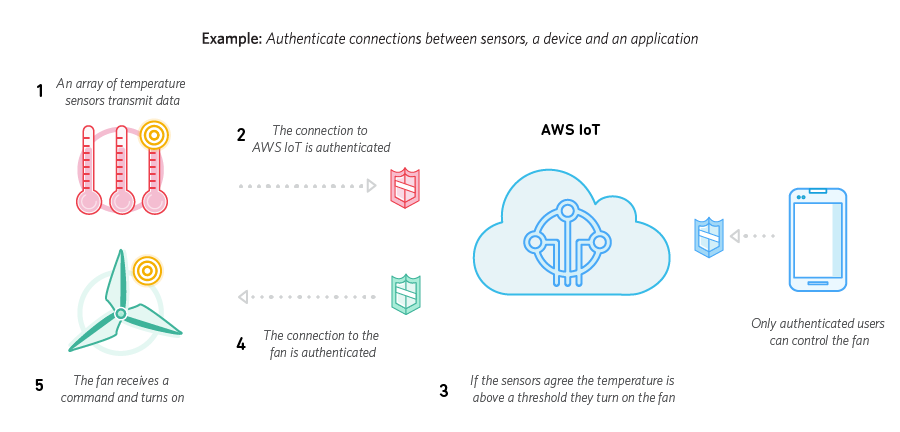
\includegraphics[width=1.0\textwidth]{content/images/IoT_Authentication.png}
	
	\caption{Kommunikation und Authentifikation von Temperatursensoren und einem Ventilator mit AWS IoT. Quelle: \cite{iot}}
	
	\label{fig:iot_authentication}
	
\end{figure}
Dementsprechend ist AWS IoT eine gute Alternative, sollte man dieses Projekt mit echten Temperatursensoren ausf�hren wollen.
\section{Funktionsweise}
Ein wichtiger Punkt bei AWS IoT ist die Sicherheit der Kommunikation zwischen den einzelnen Endpunkten. Sicherheit ist bei IoT generell ein gro�es Thema, da unter Umst�nden mit sensiblen Daten gearbeitet wird, die im eigenen Haus erzeugt werden. AWS IoT stellt sicher, dass keine Kommunikation �ber AWS IoT unverschl�sselt stattfindet, indem sich jeder Endpunkt zun�chst bei AWS IoT authentifizieren muss. Jede Kommunikation wird einzeln authentifiziert und verschl�sselt. Dies sieht man z.B. in Abbildung  \ref{fig:iot_authentication}. Hier wird in Schritt 2 die Kommunikation der Temperatursensoren mit AWS IoT authentifiziert, bevor sie die Daten an AWS IoT senden. In Schritt 4 wird die Kommunikation mit dem Ventilator ebenfalls zun�chst authentifiziert. Und nat�rlich k�nnen nur authentifizierte Nutzer �ber Mobilapplikationen �ber AWS IoT wie in diesem Beispiel den Ventilator kontrollieren.
\begin{figure}[h!]
	
	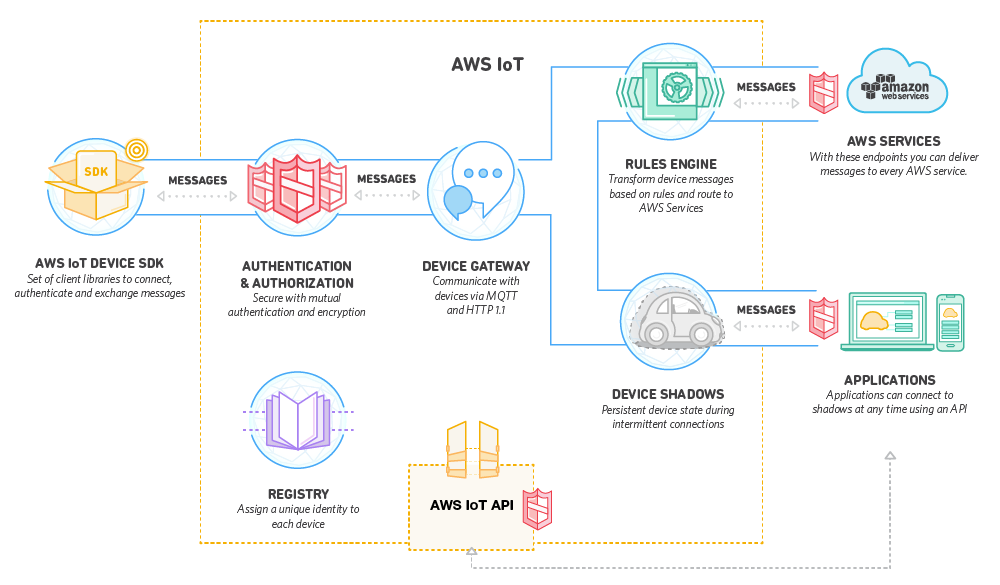
\includegraphics[width=1.1\textwidth]{content/images/IoT_Functions.png}
	
	\caption{Funktions�bersicht von AWS IoT. Quelle: \cite{iot_functions}}
	
	\label{fig:iot_functions}
	
\end{figure}

Abbildung \ref{fig:iot_functions} zeigt eine Funktions�bersicht von AWS IoT. Hier steht zun�chst einmal auf der linken Seite die AWS Device SDK, die eine Reihe von Client Libraries bereitstellt, mit der Ger�te mit AWS IoT kommunizieren k�nnen. Die Kommunikation findet dabei �ber die Protokolle MQTT \cite{mqtt} oder HTTP statt. MQTT ist ein leichtgewichtiges Nachrichtenprotokoll f�r die direkte Kommunikation zwischen Maschinen (M2M) und ist daher ein h�ufig genutztes Protokoll im Bereich des IoT. Mittels einem dieser beiden Protokolle kommuniziert das Ger�t, das die AWS Service SDK nutzt, mit dem Device Gateway. Die Kommunikation wird dabei verschl�sselt und zun�chst m�ssen sich beide Seiten auch authentifizieren, bevor �berhaupt eine Kommunikation zustande kommt. AWS IoT unterst�tzt dabei die AWS-Methode der Authentifizierung (mit der Bezeichnung ``SigV4'') sowie eine Authentifizierung auf der Basis von X.509 \cite{iot_functions}. Den Ger�ten k�nnen einzelne Richtlinien vorgegeben werden, die ihren Zugriff entsprechend einschr�nken oder es k�nnen Rollen definiert werden, die Ger�ten eine genau spezifizierte Menge an Rechten geben. \newline
Die Registry erstellt eine eindeutige Identit�t f�r die Ger�te. Diese ist f�r alle Ger�te egal welcher Art einheitlich formatiert. Au�erdem werden Metadaten von Ger�ten gespeichert, die bspw. angeben, welche Funktionen dieses Ger�t unterst�tzt wie zum Beispiel, dass ein Sensor Temperaturdaten meldet und in welcher Einheit diese Temperaturdaten �bermittelt werden. \newline
Das Device Gateway stellt f�r Applikationen REST APIs bereit, �ber die die Applikationen die Statusinformationen von Ger�ten auslesen und manipulieren k�nnen. Dazu legt das Device Gateway sogenannte ``Device Shadows'' bzw. ``Schattenger�te'' an, die den letzten Zustand des Ger�tes darstellen. Das hei�t, dass der Zustand von Ger�ten auch dann ausgelesen werden kann, wenn das Ger�t gar nicht mehr online ist, da der letzte Zustand als ``Schattenger�t'' gespeichert wurde. Zudem k�nnen Applikationen so auch den gew�nschten zuk�nftigen Zustand festlegen. Auch dieser wird im ``Schattenger�te'' persistiert und wird auf das Ger�t �bertragen, wenn es wieder online ist. Damit ist es m�glich, auch f�r Ger�te, die nicht dauerhaft online sind, eine REST API bereitzustellen, die dauerhaft verf�gbar ist und Applikationen erm�glicht, sich immer mit dem ``Schattenger�t'' zu synchronisieren und den Status zu ver�ndern. Die Kommunikation erfolgt auch hier wieder �ber verschl�sselte Nachrichten.
\begin{figure}[h!]
	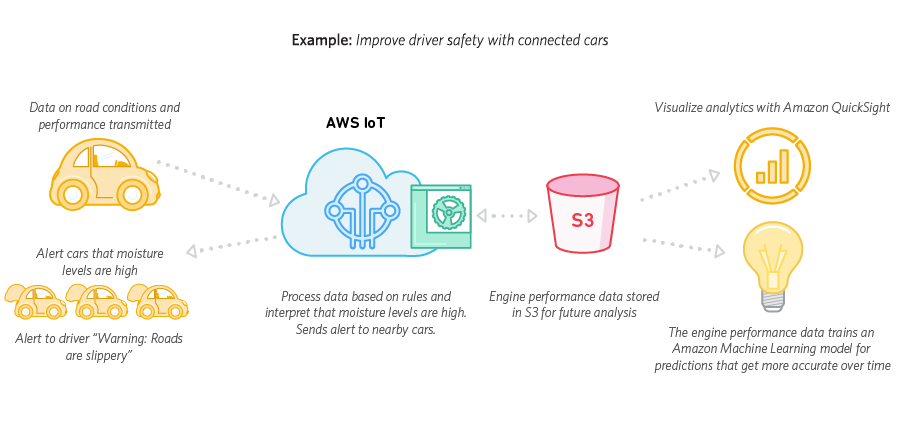
\includegraphics[width=1.1\textwidth]{content/images/IoT_S3.png}
	
	\caption{Beispiel der Kommunikation von AWS IoT mit anderen Amazon Services wie S3. Quelle: \cite{iot}}
	
	\label{fig:iot_s3}
	
\end{figure}
Das Device Gateway kann aber auch �ber die Rules Engine Daten von Ger�ten transformieren und an andere Services weiterleiten. So k�nnten beispielsweise Temperaturdaten an Amazon DynamoDB oder andere Datenbank Services weitergeleitet werden. Die Abbildung \ref{fig:iot_S3} zeigt die Kommunikation von AWS IoT mit Amazon S3, bei der Performance Daten von Autos �ber AWS IoT an S3 �bermittelt und zur weiteren Auswertung gespeichert werden.  \newline
Es k�nnen aber auch Regeln erstellt werden, die bei bestimmten Konditionen Aktionen ausl�sen. Zum Beispiel k�nnte beim �berschreiten einer bestimmten Menge an Temperaturen eine Nachricht an AWS Lambda \cite{lambda} geschickt werden, das daraufhin den Mittelwert der gesammelten Daten berechnet. Nachrichten k�nnen aber auch an Ger�te geschickt werden wie in Abbildung \ref{fig:iot_authentication}. Erreicht die Temperatur der Sensoren einen Grenzwert, greift eine Regel und sendet den Befehl an den Ventilator, der sich daraufhin einschaltet. \newline
Die Regeln werden direkt in der Management Konsole eingetragen oder �ber eine SQL-�hnliche Syntax definiert.  \newline
AWS IoT bietet also passende Funktionen, um das Projekt mit echten Temperatursensoren umzusetzen. Man k�nnte die Temperaturdaten direkt an einen Datenbank Service wie Amazon DynamoDB weiterleiten und auch die Temperatursensoren �ber die REST API direkt steuern. Mittels der Rules Engine k�nnten Regeln festgelegt werden, nach denen bei bestimmten Temperaturen bestimmte Aktionen ausgef�hrt werden k�nnen. Dadurch k�nnte man auch andere Ger�te wie beispielsweise Ventilatoren oder Klimaanlagen einbinden und mittels AWS IoT steuern lassen. Man ben�tigt aber neben den Sensoren auch Mikrocontroller wie bspw. Raspberry PIs \cite{raspberry}, die mit den Sensoren und anderen Ger�ten kommunizieren k�nnen, um AWS IoT nutzen zu k�nnen.  \newline \newline


\section{AWS IoT CLI, SDK und APIs}
Die AWS IoT CLI bietet die M�glichkeit �ber Kommandozeileneingaben verschiedene Funktionen von AWS IoT zu nutzen. Beispielsweise k�nnen Ger�te zur Device Registry hinzugef�gt werden und Eintr�ge in der Registry ver�ndert werden. 

\lstinputlisting[firstline=1, lastline=1, caption=Einf�gen eines Ger�ts in die Registry. Quelle: \cite{iot_registry} , label=iot_describe_1, style=java]{content/listings/iot_describe.txt}

Der Quellcode \ref{iot_describe_1} zeigt den Befehl, mit dem ein Ger�t mit dem Namen ``MyDevice3'' in die Registry eingef�gt werden kann.

\lstinputlisting[firstline=2, lastline=10, caption=Ger�teeintrag in der Registry. Quelle: \cite{iot_registry} , label=iot_describe_2, style=java]{content/listings/iot_describe.txt}

Der Eintrag in der Registry sieht dann wie in Quelltext \ref{iot_describe_2} aus. Weitere Attribute wie eine einzigartige Seriennummer werden automatisch generiert. \newline
Die AWS IoT CLI bietet zudem auch die M�glichkeit alle Ger�te in der Registry anzuzeigen oder die Suchergebnisse zu filtern. \newline
Mittels SDK lassen sich auch Regeln erstellen, einsehen und bearbeiten.

\lstinputlisting[firstline=1, lastline=1, caption=Erstellen einer AWS IoT Regel. Quelle: \cite{iot_rules} , label=iot_rule_1, style=java]{content/listings/iot_create_rule.txt}

In Quelltext \ref{iot_rule_1} wird eine Regel mit dem Namen ``my-rule'' erzeugt. Zudem wird eine payload Datei namens ``my-rule.json'' ebenfalls mitgeschickt.

\lstinputlisting[firstline=2, lastline=15, caption=Inhalt einer Payload Datei. Quelle: \cite{iot_rules} , label=iot_rule_2, style=java]{content/listings/iot_create_rule.txt}

Die Payload Datei in Quelltext \ref{iot_rule_2} enth�lt die Regel, alle Nachrichten, die an die Topic ``iot-topic'' gesendet werden, in die DynamoDB Tabelle ``my-dynamodb-table'' zu schreiben. Dabei wird noch eine Rolle �bergeben, die in diesem Fall das Recht hat, auf die DynamoDB Tabelle zuzugreifen und in diese zu schreiben. Als HashkeyValue wird der Name der Topic �bergeben und als rangeKeyValue der Timestamp der Nachricht.

\lstinputlisting[firstline=1, lastline=1, caption=GET Anfrage an einen ``Ger�teschatten''. Quelle: \cite{iot_get_thingshadow} , label=iot_get_shadow_1, style=java]{content/listings/iot_get_thingshadow.txt}

Mittels einer REST API k�nnen die ``Ger�teschatten'' von Ger�ten abgefragt und auch manipuliert werden. Quelltext  \ref{iot_get_shadow_1} zeigt eine HTTP GET Anfrage an einen Ger�teschatten, wobei ``endpoint'' und ``thingName'' Variablen sind, die man in der AWS IoT Konsole auslesen kann oder auch per AWS IoT SDK.

\lstinputlisting[firstline=2, lastline=3, caption=GET Antwort auf die Anfrage an einen ``Ger�teschatten''. Quelle: \cite{iot_get_thingshadow} , label=iot_get_shadow_2, style=java]{content/listings/iot_get_thingshadow.txt}

Quelltext  \ref{iot_get_shadow_2} zeigt die Antwort auf eine Anfrage an einen ``Ger�teschatten''. ``response state document'' ist hierbei ein gr��eres Dokument, das Informationen �ber den Status des ``Ger�teschattens'' sowie Metadaten, einen Timestamp und andere Informationen enth�lt. \newline
�ber die API ist es auch m�glich, ``Ger�teschatten'' zu bearbeiten und zum Beispiel einen neuen Status zu setzen, der dann im Ger�t gesetzt wird, wenn es online ist oder auch ``Ger�teschatten'' zu l�schen. \newline
Es gibt au�erdem noch eine AWS IoT SDK \cite{iot_sdk}, die die Integration von Ger�ten in AWS IoT vereinfacht. Die SDK ist f�r C, Arduino Y�n \cite{arduino_yun} und Node.js \cite{nodejs} verf�gbar. \newline
Sie bietet Funktionen zum Anmelden der Ger�te bei AWS IoT, dem Aufbauen von Verbindungen und Senden von Nachrichten �ber die Verbindung sowie zum Bearbeiten von ``Ger�teschatten''.

\section{Zusammenfassung}
IoT wird ein wichtiger Teil der IT in den n�chsten Jahren sein und AWS IoT kann helfen, IoT auch dem Massenmarkt verf�gbar zu machen. Im Weg stehen im Moment die geringe Einsteigerfreundlichkeit der zu AWS IoT kompatiblen Ger�te. Direkt kompatibel sind nur einige von Amazon angebotene Ger�te und auch dort ist noch eine Menge Konfigurationsarbeit n�tig. Die Dokumentation dieser Ger�te ist leider bisher auch nicht allzu gut und es lassen sich nur wenige Erfahrensberichte finden. Da AWS IoT Stand Februar 2016 allerdings auch erst einen Monat offiziell nutzbar ist, kann sich dies im Laufe der Zeit noch �ndern. Wenn AWS IoT in der Zukunft auch mit weniger Aufwand betreibbar ist, kann es ein wichtiger Teil des IoT Marktes werden.
	\chapter{Evaluation}
	In diesem Kapitel werden die genutzten Amazon Web Services Kinesis und DynamoDB betrachtet und deren Nutzen f�r ein Projekt dieser Art evaluiert. Zudem wird der potentielle Nutzen von AWS IoT bei Nutzung echter Sensoren evaluiert und noch einige andere Implementierungsm�glichkeiten betrachtet.
\section{Evaluation Kinesis und DynamoDB}
\label{eva_kinesis}
Amazon Kinesis war in diesem Projekt eine sehr wichtige Komponente, die es erm�glichte das Projekt schnell durchzuf�hren, aber auch gute Ergebnisse erzielen zu k�nnen. Kinesis ist leicht nutzbar und bietet einen guten Durchsatz der Daten. So war es ohne Probleme m�glich mehrere tausend Temperaturdaten von verschiedenen Sensoren pro Sekunde �ber Amazon Kinesis zu �bertragen und zu verarbeiten. Dabei wurde zur Vereinfachung ein einfacher kommaseparierter String erzeugt, der die Temperaturdaten enthielt, und mittels Amazon Kinesis �bertragen. Dieser String wurde vom Consumer verarbeitet und die Temperaturdaten dann manuell in DynamoDB persistiert. Es ist aber auch m�glich, eigene Modelklassen f�r die Daten zu erstellen und mittels Annotationen direkt anzugeben, welches Attribut ein Key Attribut ist usw. und die Modelklasse direkt auf DynamoDB zu persistieren. F�r das vergleichsweise einfache Datenmodell dieses Projekts war dies nicht notwendig, aber f�r komplexere Projekte ist das ein gro�er Vorteil. Zudem wurde in diesem Projekt ein Kinesis Stream mit nur einem einzigen Shard genutzt. F�r gr��ere Projekte k�nnen mehr Shards genutzt werden, die den Datendurchsatz noch weiter erh�hen k�nnen.\newline
Die Nutzung von DynamoDB war in diesem Projekt ebenfalls recht einfach. Es mussten zu jedem Temperaturwert ein Hashkey sowie ein Rangekey angegeben werden, die eigentlichen Temperaturwerte konnten dann direkt in diesem Datensatz gespeichert werden. Auch eine Map kann in DynamoDB so direkt und ohne Anpassung des Formats im Gegensatz zu relationalen Datenbanken in diesem Datensatz gespeichert werden . Zudem war DynamoDB in den Testphasen recht performant und konnte mehrere tausend Datens�tze pro Sekunde persistieren. Hier war es allerdings notwendig das Datenformat etwas anzupassen und pro Sensordurchlauf nur noch einen Datensatz zu erstellen und die einzelnen Temperaturwerte als Map in diesem Datensatz zu speichern und diesen Datensatz nur noch zu bearbeiten. Wurden alle Datens�tze einzeln persistiert, konnte DynamoDB nur noch einige hundert Temperaturen pro Sekunde maximal persistieren. Trotz gutem Datendurchsatz ist ein passendes Datenmodell also dennoch wichtig f�r eine gute Performance von DynamoDB. \newline
Ein negativer Punkt in Sachen Kinesis ist die permanente Speicherung der Daten innerhalb eines Kinesis Streams. Daten, die �ber einen Kinesis Stream gesendet werden, werden noch bis zu einer Woche gespeichert, damit sie weiterhin von einem Consumer gelesen werden k�nnen. Das ist zun�chst einmal ein positiver Punkt, allerdings ist die Speicherung vergleichsweise kostenintensiv. Wurde ein Stream nach Einsatz nicht gel�scht, wurden die �bertragenen Daten im Stream persistiert, was schon nach wenigen Tagen Kosten von mehreren Dollar zur Folge hatte. F�r dieses Projekt mit dieser Datenmenge kein Problem, da ja auch ein gewisses Budget gew�hrt worden war, bei gr��eren Projekten k�nnen dadurch aber unter Umst�nden gr��ere Kosten entstehen, die aber vollkommen unn�tig sind. Im Laufe dieses Projekts wurde keine M�glichkeit gefunden, die Persistierung der Daten in Streams schon im Vorhinein zu unterbinden, was das Monitoring der Amazon Web Services und besonders von Amazon Kinesis sehr wichtig machte, um keine unn�tigen Kosten zu verursachen. \newline
Positiv zu erw�hnen ist, dass die �bertragung der Daten �ber Kinesis in den Tests immer kostenlos war, da sich die Datenmenge noch im kostenlosen Bereich von Kinesis befand. Um innerhalb dieses Bereichs zu bleiben, wurden die Producer bewusst nur maximal einige Minuten betrieben. Bei dauerhaftem Einsatz w�rde die Datenmenge auch in den kostenpflichtigen Bereich steigen. Genauso waren auch die Kosten f�r die Nutzung von DynamoDB und Amazon EC2 im Cent- oder maximal im niedrigen Dollarbereich. \newline
Ein weiterer positiver Punkt ist die recht gute Dokumentation der verschiedenen Webservices von Amazon, die einen schnellen Einstieg erm�glicht. Die Grundlagen aller Services sind gut erkl�rt und auch die APIs und Client Libraries werden beschrieben. Besonders die Beispielprojekte einzelner Services sind ein guter Einstieg in AWS. Negativ ist, dass die Dokumentation �ber die Grundlagen meist nicht hinaus geht und im Bereich Amazon Kinesis die Kinesis Connectors nur sehr kurz beschrieben wurden, so dass diese in diesem Projekt nicht genutzt werden konnten, da es aufgrund der geringen Dokumentation zu viel Zeit gebraucht h�tte die Funktionsweise dieser Library zu verstehen. \newline
Die Nutzung von Docker war im Rahmen dieses Projektes auch sehr simpel umzusetzen, da es von vornherein als Maven Projekt geplant wurde, f�r das es ein eigenes Docker Image gibt. Somit war nur wenig Arbeit notwendig, um das Projekt in einem Docker Container zu starten und damit war auch das Deployment auf Amazon EC2 mittels Amazon ECS kein Problem mehr. Mit Amazon ECS lassen sich in Docker Container gepackte Applikationen direkt auf Amazon EC2 deployen, was eine effiziente M�glichkeit f�r dieses Projekt darstellte. 
\section{Evaluation AWS IoT}
AWS IoT ist eine Service von Amazon, der zwar nicht in diesem Projekt verwendet wurde, im Rahmen dieses Themas aber so interessant ist, dass er trotzdem als weitere Alternative betrachtet werden sollte. Es bietet eine Plattform, �ber die IoT Ger�te wie bspw. Sensoren miteinander kommunizieren k�nnen sowie AWS IoT auch mit den Ger�ten kommunizieren kann (s. Kapitel \ref{aws_iot}). \newline
In diesem Projekt k�nnte AWS IoT die Rolle von Amazon Kinesis als Kommunikationsweg der Sensoren �bernehmen mit dem Unterschied, dass IoT direkt f�r physikalische Ger�te entwickelt wurde. Wenn man also physikalische Ger�te einsetzen m�chte, k�nnte AWS IoT die effizientere L�sung sein. \newline
Vorteile sind also die M�glichkeit der direkten Anbindung physikalischer Ger�te sowie die simple Kommunikationsm�glichkeit zwischen den Ger�ten. Zudem ist eine Anbindung an weitere Amazon Services wie bspw. DynamoDB zur Datenhaltung m�glich. \newline
Negativ ist vor allem die geringe Anzahl der zu AWS IoT direkt kompatiblen Ger�te sowie die bisher recht geringe Dokumentation dieser Ger�te. Daher ist ein Einstieg im Moment nicht allzu einfach und mit einiger Konfigurationsarbeit verbunden. Eventuell k�nnte sich dieser Zustand zuk�nftig aber noch �ndern, vor allem im Hinblick darauf, dass AWS IoT noch nicht allzulange verf�gbar ist.
\section{Evaluation anderer Implementierungsm�glichkeiten}
Bei der Ausf�hrung dieses Projektes wurden noch einige andere Implementierungsm�glichkeiten ins Auge gefasst, die allerdings aus verschiedenen Gr�nden in diesem Projekt nicht umgesetzt werden konnten. \newline
Dazu z�hlen zum einen die bereits in Kapitel \ref{eva_kinesis} erw�hnten Kinesis Connectors. Diese h�tten die Projektarchitektur erheblich ver�ndert und den Consumer �berfl�ssig gemacht. Vorteil dieser Variante w�re gewesen, dass die �bermittlung der Daten direkt �ber Kinesis an DynamoDB gelaufen w�re ohne den Umweg �ber den Consumer, was die Aktualit�t der Daten n�her an Echtzeit herangebracht h�tte, welches eine der geplanten Anforderungen darstellt. \newline
Eine weitere M�glichkeit w�re die Nutzung anderer Datenbanksysteme gewesen. Amazon bietet neben DynamoDB zudem noch Amazon RDS an. Eine L�sung mit RDS w�re ebenfalls m�glich gewesen, da das Datenmodell so simpel ist, dass auch relationale Datenbanken voraussichtlich eine �hnliche Performance h�tten liefern k�nnen. Eine eigene L�sung bspw. mit Apache Cassandra wurde ebenfalls er�rtert, letztendlich aufgrund von Zeitmangel aber verworfen. Es wurde auf die L�sung mit DynamoDB gesetzt, um eine weitere neue Technologie kennen zu lernen und weil diese Technologie gute Performance liefert und dank guter Dokumentation einen leichten Einstieg bot. \newline
Eine Anforderung an das Projekt war die Nutzer mehrerer AWS Services, um die unterschiedlichen AWS Services im Rahmen des Projektes evaluieren zu k�nnen, im Besonderen bei der Verwendung von gro�en Datenstr�men. Hier h�tte sich beispielsweise eine eigene L�sung mit Amazon EC2 angeboten, die allerdings f�r dieses Projekt zu komplex gewesen w�re. Es h�tten die Funktionen von Amazon Kinesis selbst umgesetzt werden k�nnen, was bei der Zuverl�ssigkeit von Amazon Kinesis innerhalb des Projekts aber auch nicht notwendig ist.
\section{Zusammenfassung}
Insgesamt kann also gesagt werden, dass die genutzen Amazon Web Services f�r gro�e Datenstr�me gut geeignet sind. Im Test konnten mehrere tausend Temperaturdaten innerhalb einer Sekunde �bermittelt werden und es kann immer noch nach oben skaliert werden f�r einen wesentlich h�heren Datendurchsatz. F�r dieses Projekt war die Dokumentation der AWS Services recht gut, k�nnte in einigen Punkten aber noch etwas weiter gehen.

	\chapter{Fazit}

Das Projekt verlief insgesamt recht gut und es konnten alle entscheidenden Anforderungen an das Projekt umgesetzt werden. Die Evaluation der genutzten Amazon Web Services zeigte, dass sie f�r die Verarbeitung gr��erer Datenstr�me geeignet sind und auch bei gr��erem Datendurchsatz eine gute Performance bieten. Dies bezieht sich besonders auf AWS Kinesis, das die �bertragung der Temperaturdaten stark vereinfachte. Zudem zeigte sich auch eine gute Einsteigerfreundlichkeit bei der Nutzung der Client SDKs durch eine gute Dokumentation, die allerdings bei weiterf�hrenden Themen nicht immer so umfangreich war. Daher war es im Rahmen dieses Projektes leider nicht m�glich, einige Technologien zu nutzen, die weitere Erkenntnisse zu AWS h�tten bringen k�nnen. \newline
Positiv ist zudem die Projektplanung und insbesondere die Risikoplanung zu nennen, durch die einige Risiken abgeschw�cht werden konnten und das Projektziel somit nicht gef�hrdet wurde. Auch das Budget konnte dank der dauerhaften �berwachung der Kosten eingehalten werden, obwohl einige unerwartete Kosten anfielen. \newline
Die Integration des Projektes in ein Docker Image war dank der vorhandenen passenden Basisimages wie dem hier genutzten Maven Image ebenfalls sehr einfach und konnte gut umgesetzt werden. \newline
Zudem wurde in AWS IoT ein neuer Amazon Web Service evaluiert, der f�r die Nutzung von echten Sensoren konzipiert wurde und damit auch einen Blick in den potentiellen IoT-Markt der Zukunft erm�glicht. Hier kann ein generell positives Fazit gezogen werden, da AWS IoT einige Funktionen bietet, die die Kommunikation mit IoT-Ger�ten vereinfacht und die Integration von anderen Amazon Web Services zur Datenhaltung oder Verarbeitung der Daten erm�glicht. \newline
Zuk�nftig k�nnte dieses Projekt  entsprechend der bisher nicht umgesetzten Anforderungen erweitert werden oder die bisher umgesetzten Klassen k�nnten anders implementiert werden, um weitere Funktionen von Amazon Web Services zu testen.
	
	% ----------------- Ende des eigentlichen Textes
	
	
	%Verzeichnisse erstellen
  	\chapter*{Abk�rzungsverzeichnis}
\begin{acronym}[BiPRO ] %L�ngster Begriff
\setlength{\itemsep}{-\parsep}
	\acro{AWS}{Amazon Web Services}
	\acro{EC2}{Amazon Elastic Compute Cloud}
	\acro{ECS}{Amazon EC2 Container Service }
	\acro{HTTP}{Hypertext Transfer Protocol}
	\acro{IoT}{Internet of Things}
	\acro{RDS}{Amazon Relational Database Service}
	\acro{REST}{Representational State Transfer}
	%usw.
\end{acronym}

	\listoffigures
	\listoftables
	\lstlistoflistings
	
	\appendix
	\nocite{*} 
	
	%Literaturverzeichnis einbinden:
	\begin{thebibliography}{1}


\bibitem{projektarbeit}
Hendrik Hagmans, ``Projektarbeit Evaluierung einer Amazon Web Services Lösung zur Erfassung und Verarbeitung von Sensordaten''; im Rahmen des WS 15 an der FH Dortmund, abgerufen am 28. Oktober 2015

\bibitem{iot_vision}
Daniele Miorandi, Sabrina Sicari, Francesco De Pellegrini, Imrich Chlamtac, ``Internet of things: Vision, applications and research challenges''; \url{https://irinsubria.uninsubria.it/retrieve/handle/11383/1762288/2389/IOT.pdf}, abgerufen am 28. Oktober 2015

\bibitem{aws}
Amazon Inc, ``Amazon Web Services''; \url{http://aws.amazon.com/de/}, abgerufen am 28. Oktober 2015

\bibitem{docker}
Docker Inc, ``Docker''; \url{https://www.docker.com/}, abgerufen am 28. Oktober 2015

\bibitem{ecs}
Amazon Inc, ``Amazon ECS''; \url{http://aws.amazon.com/de/ecs/}, abgerufen am 28. Oktober 2015

\bibitem{ec2}
Amazon Inc, ``Amazon EC2''; \url{http://aws.amazon.com/de/ec2/}, abgerufen am 28. Oktober 2015

\bibitem{rds}
Amazon Inc, ``Amazon RDS''; \url{http://aws.amazon.com/de/rds/}, abgerufen am 28.
Oktober 2015

\bibitem{dynamodb}
Amazon Inc, ``Amazon Dynamo DB''; \url{http://aws.amazon.com/de/dynamodb/}, abgerufen am 28. Oktober 2015

\bibitem{kinesis}
Amazon Inc, ``Amazon Kinesis''; \url{http://aws.amazon.com/de/kinesis/}, abgerufen am 28. Oktober 2015

\bibitem{kinesisconnector}
Amazon Inc, ``Amazon Kinesis Connector Library''; \url{https://github.com/awslabs/amazon-kinesis-connectors}, abgerufen am 28. Oktober 2015

\bibitem{firehose}
Amazon Inc, ``Amazon Kinesis Firehose''; \url{https://aws.amazon.com/de/firehose/}, abgerufen am 28. Oktober 2015

\bibitem{s3}
Amazon Inc, ``Amazon S3''; \url{https://aws.amazon.com/de/s3/}, abgerufen am 28. Oktober 2015

\bibitem{kinesis_sample_1}
Amazon Inc, ``Amazon Kinesis Data Visualization Sample Application''; \url{https://github.com/awslabs/amazon-kinesis-data-visualization-sample}, abgerufen am 28. Oktober 2015

\bibitem{kinesis_sample_2}
Amazon Inc, ``KPL Java Sample Application''; \url{https://github.com/awslabs/amazon-kinesis-producer/tree/master/java/amazon-kinesis-producer-sample}, abgerufen am 28. Oktober 2015

\bibitem{lambda}
Amazon Inc, ``AWS Lambda''; \url{http://aws.amazon.com/de/lambda/}, abgerufen am 28. Oktober 2015

\bibitem{iot}
Amazon Inc, ``AWS IoT''; \url{http://aws.amazon.com/de/iot/}, abgerufen am 28. Oktober 2015


\bibitem{iot_functions}
Amazon Inc, ``AWS IoT Funktionsweise''; \url{https://aws.amazon.com/de/iot/how-it-works/}, abgerufen am 28. Oktober 2015

\bibitem{iot_registry}
Amazon Inc, ``AWS IoT Thing Registry''; \url{http://docs.aws.amazon.com/iot/latest/developerguide/thing-registry.html}, abgerufen am 28. Oktober 2015

\bibitem{iot_rules}
Amazon Inc, ``AWS IoT Creating an AWS IoT Rule''; \url{http://docs.aws.amazon.com/iot/latest/developerguide/aws-iot-create-rule.html}, abgerufen am 28. Oktober 2015

\bibitem{iot_get_thingshadow}
Amazon Inc, ``AWS IoT GetThingShadow''; \url{http://docs.aws.amazon.com/iot/latest/developerguide/API_GetThingShadow.html}, abgerufen am 28. Oktober 2015

\bibitem{iot_sdk}
Amazon Inc, ``AWS IoT SDK''; \url{http://docs.aws.amazon.com/iot/latest/developerguide/iot-sdks.html}, abgerufen am 28. Oktober 2015

\bibitem{mqtt}
MQTT Org, ``MQTT''; \url{http://mqtt.org/}, abgerufen am 28. Oktober 2015

\bibitem{raspberry}
Raspberry Pi Foundation, ``Raspberry PI''; \url{https://www.raspberrypi.org/}, abgerufen am 28. Oktober 2015

\bibitem{cassandra}
Apache Software Foundation, ``Apache Cassandra''; \url{http://cassandra.apache.org/}, abgerufen am 28. Oktober 2015

\bibitem{maven}
Apache Software Foundation, ``Apache Maven''; \url{https://maven.apache.org/}, abgerufen am 28. Oktober 2015

\bibitem{maven_image}
Apache Software Foundation, ``Apache Maven Image''; \url{https://hub.docker.com/_/maven/}, abgerufen am 28. Oktober 2015

\bibitem{jetty}
Eclipse Foundation, ``Eclipse Jetty''; \url{http://www.eclipse.org/jetty/}, abgerufen am 28. Oktober 2015

\bibitem{nodejs}
Node.js Foundation, ``Node.js''; \url{https://nodejs.org/en/}, abgerufen am 28. Oktober 2015

\bibitem{canvasjs}
fenopix, ``CanvasJS''; \url{http://canvasjs.com/}, abgerufen am 28. Oktober 2015

\bibitem{arduino_yun}
Arduino Foundation, ``Arduino Yún''; \url{https://www.arduino.cc/en/Main/ArduinoBoardYun}, abgerufen am 28. Oktober 2015

\bibitem{kinesis_concepts}
Amazon Inc, ``Amazon Kinesis Key Concepts'';  \url{http://docs.aws.amazon.com/kinesis/latest/dev/key-concepts.html}, abgerufen am 28. Oktober 2015

\end{thebibliography}
	%\chapter{Anhang}
\Blindtext[4]

\end{document}
